\documentclass[journal,12pt,twocolumn]{IEEEtran}
\usepackage[utf8]{inputenc}
\usepackage{amsmath}
\usepackage{listings}
\usepackage{physics}
\newcommand{\myvec}[1]{\ensuremath{\begin{pmatrix}#1\end{pmatrix}}}
\let\vec\mathbf
\usepackage{graphicx}
\graphicspath{ {./images/} }

\title{Assignment 2
\\Probability }
\author{Swati Mohanty (EE20RESCH11007) }
\date{September 2020}

\begin{document}

\maketitle


\section{Problem}
A die is thrown three times. Events A and B are defined as below:
\\A : 4 on the third throw.
\\B : 6 on the first and 5 on the second throw.
\\Find the probability of A given that B has
already occurred?
\section{Solution}
Total sample space =216
\\Sample space of A (4 on the third throw) = 36
\\Sample space of B (6 on the first and 5 on  second throw) = 6
\begin{align}
    P(A) = \frac{36}{216}
    \\
    P(B) = \frac{6}{216}
    \\
P(A\cap B) = P(A) \times P(B)  
\\= \frac{36}{216} \times \frac{6}{216} = \frac{1}{216}
\\
    P(A | B) = \frac{P(A\cap B)}{P(B)}
    \\
    =\frac{\frac{1}{216}}{\frac{6}{216}} = \frac{1}{6} = 0.167
\end{align}
\section{Simulation result}
Theoretical probability = 0.167
\\Simulated probability = 0.162
\\Percetage of error obtained = 3.02%
\\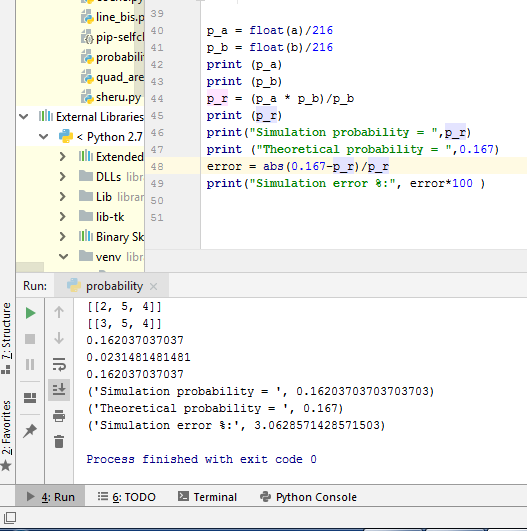
\includegraphics[width=10cm, height=10cm]{simulation result.png}
\\Python project link 
\begin{lstlisting}
https://github.com/Swati-Mohanty/EE5600/tree/master/Assignment%202
\end{lstlisting}
\end{document}